\chapter{Preparation}

\section{The CTSP is at Least as Hard as the DTSP}

This section contains a proof that the CTSP is at least as hard as the DTSP. This structure of the proof will be:
\begin{enumerate}
  \item Consider an arbitrary instance of the DTSP $(V,C)$
  \item Transform this into an instance of the CTSP $(D,P,f,t)$
  \item Assume we can find an optimal solution $L$ to the CTSP instance
  \item Transform $L$ into a solution $T$ of the DTSP instance
  \item Show that $T$ is optimal
\end{enumerate}

This proof, taken alongside the fact that the DTSP is NP-hard\cite{Korte2008}, will prove that the CTSP is NP-hard. The proof is below.

\begin{quote}
  Let $(V, C)$ be an arbitrary instance of the DTSP.

  Let $D=\mathbb{R}^n$ where $n=\left|V\right|$

  Let $P=$ the set of unit basis vectors in $D$ such that $S_i=$ the $i$\textsuperscript{th} vector whose components are all 0 except for component $i$ which is 1.

  Let $V'=$ some arbitrary permutation (disallowing repetition) of $V$ such that $V_i=$ the $i$\textsuperscript{th} element.

  Let $f(x) = \begin{cases}
    \frac{C(V'_i, V'_j)}{\sqrt{2}}& \textrm{if $x$ is in the $ij$ plane, in between $P_i$ and $P_j$}\\ 
    \textrm{arbitrarily large}& \textrm{otherwise} 
   \end{cases}$
   
  Let $t(x,y) = \begin{cases}
    0& \textrm{if }x=y\\ 
    \textrm{arbitrarily large}& \textrm{otherwise} 
   \end{cases}$

  Since $f$ and $t$ must both be continuous, the \textit{arbitrarily large} value in the second cases can be continuously and rapidly increasing away from points matching the first cases. This concept is shown for $f$ in \ref{fig:dtsp-to-ctsp}.

  We then have an instance of the CTSP, $(D,P,f,t)$. Suppose we can find an optimal solution $L$.

  There exists a subset $\mathcal{L}_1$ of such solutions in which the paths consist solely of a finite number of straight line segments directly between unit basis vectors.

  Consider one such line segment in a solution $L_1 \in \mathcal{L}_1$ between arbitrary unit basis vectors $P_i$ and $P_j$. The cost of travelling along that line segment, $F_{ij}$ is:

  \begin{align}
    F_{ij} &= \int_{S_i}^{S_j} f(\mathbf{s})\;d\mathbf{s}\\
    &= \int_{S_i}^{S_j} \frac{C(V_i, V_j)}{\sqrt{sqrt{2}}}\;d\mathbf{s}\\
    &= \frac{C(V_i, V_j)}{\sqrt{sqrt{2}}} \times \left|S_i-S_j\right|\\
    &= C(V_i, V_j)\label{eq:1}
  \end{align}

  As such, the total cost $F$ of travelling along $L_1$ is bounded above by $\sum_{c\in C}c$.

  Now consider a solution $L_2 \notin \mathcal{L}_1$. By definition, $L_2$ passes through some point $x$ which is not on a diagonal line between two unit basis vectors. By the definition of $f$, the cost density at this point can be arbitrarily large, and therefore so will the total cost $F$ of travelling along $L_2$.

  There also exists a subset $\mathcal{L}_2$ of solutions which pass through every unit basis vector. By the definition of the $t$, every solution $L_3 \in \mathcal{L}_2$ will have $T=0$.

  Consider instead a solution $L_4 \notin \mathcal{L}_2$. By the definition, there must exist a unit basis vector $P_i$ which $L_4$ does not pass through. By definition of $t$, $\min_{x\in L_4} t(P_i, x)$ is arbitrarily large. As such, $L_4$ will have an arbitrarily large value of $T$.

  From these observations we can see that $\forall L' \in \mathcal{L}_1 \cap \mathcal{L}_2$, $C' \leq \sum_{c\in C}c$, and $\forall L'' \notin \mathcal{L}_1 \cap \mathcal{L}_2$, $C'$ is arbitrarily large.

  Therefore, (we can define the arbitrary largeness of $f$ and $t$ to be such that) given that $L$ is optimal, it follows that $L\in\mathcal{L}_1 \cap \mathcal{L}_2$.

  By the definition of $\mathcal{L}_1$, $L$ will consist of a finite series of diagonal line segments between unit basis vectors. Picking one such arbitrary vector $P_i$ as a starting point, these line segments can be followed to create a sequence of unit basis vectors $(P_i, P_j, P_k, \hdots)$. By the definition of $L$ we know that $L$ is a closed loop, and so we can terminate this sequence when the loop returns to the start. Furthermore, by the definition of $\mathcal{L}_2$, we know that every unit basis vector must appear in this sequence at least once.

  From this sequence, we construct a corresponding sequence $T = (V_i, V_j, V_k, \hdots)$. This is a solution to the instance of the DTSP.

  By equation \ref{eq:1} and the definition of $\hat{C}$, the total cost $C'$ of $L$ will be equal to the total cost $\hat{C}$ of $T$. We have assumed that $L$ minimizes $C'$, and so $T$ must minimize $\hat{C}$. Therefore, $T$ is an optimal solution to the instance of the DTSP.

  $\blacksquare$

\end{quote}

\begin{figure}[H]
  \centering
  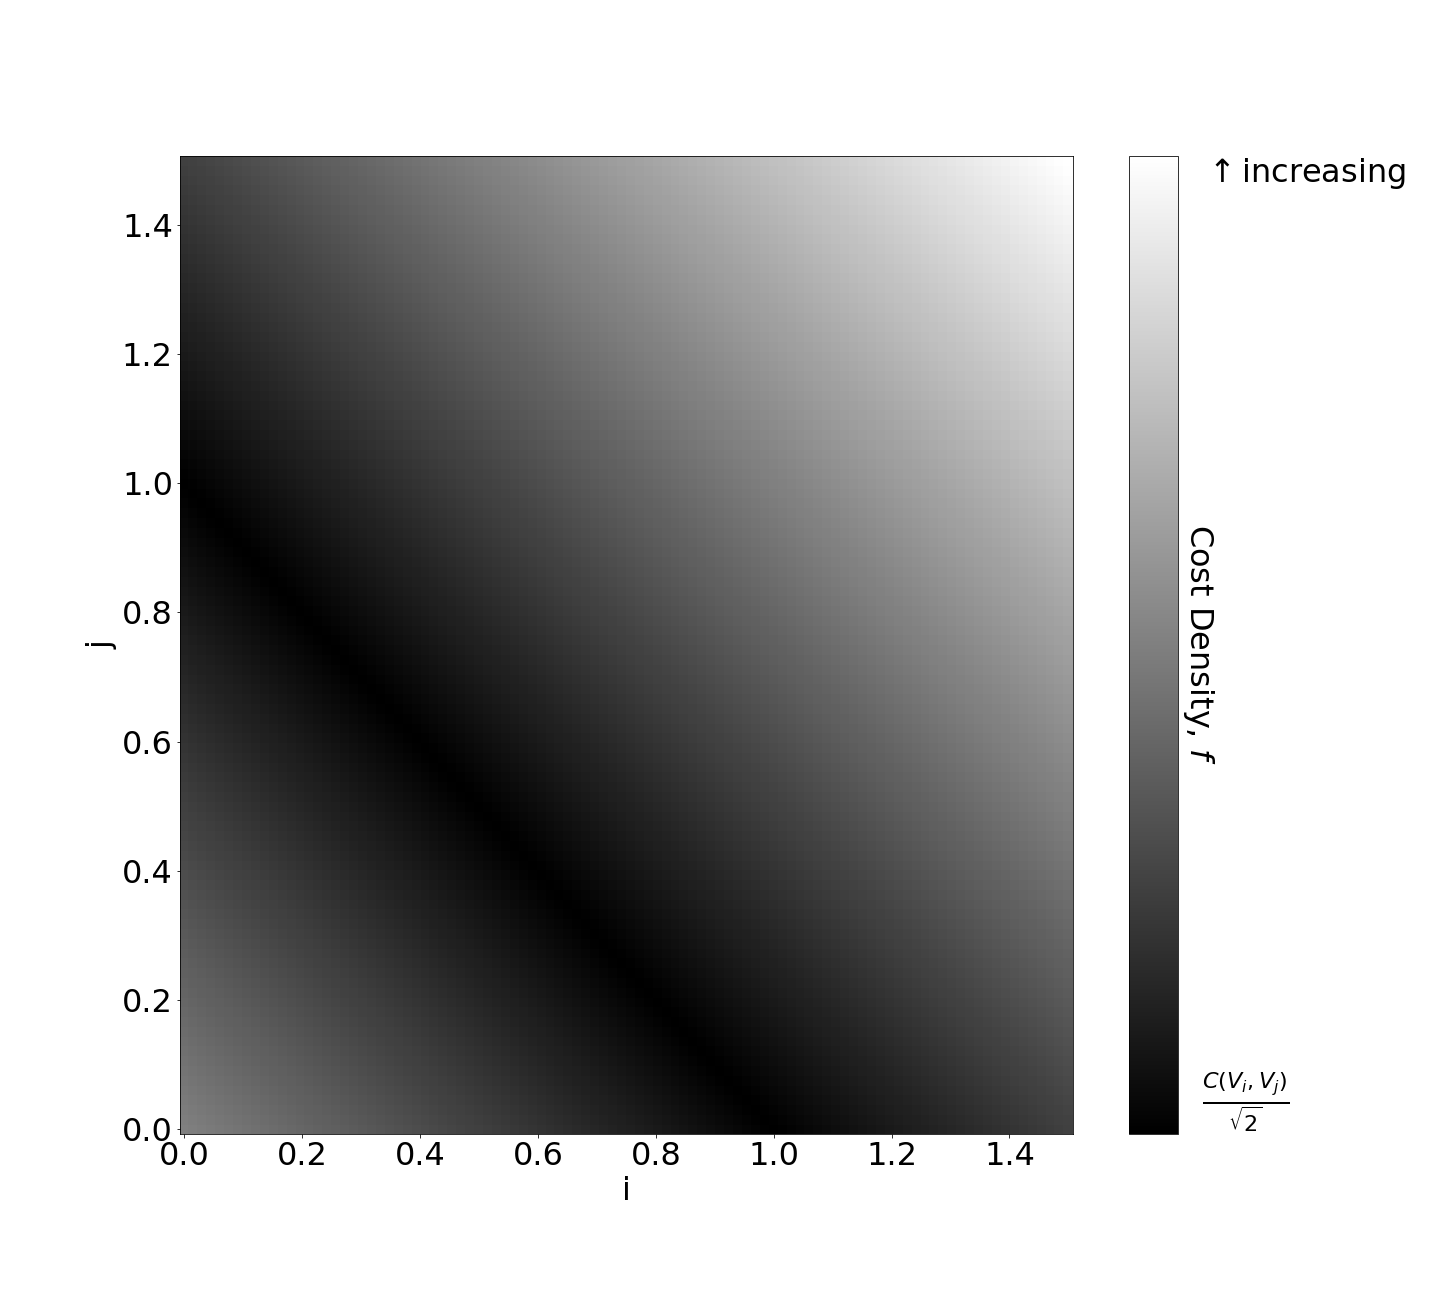
\includegraphics[width=0.5\textwidth]{dtsp-to-ctsp.png}
  \caption{\todo[caption]}
  \label{fig:dtsp-to-ctsp}
\end{figure}

\section{A Survey of DTSP Algorithms}

